\documentclass[a4paper,11pt]{article} 
\usepackage{fancyhdr}
\usepackage{polski}
\usepackage{graphicx}
\usepackage{tabularx}
\usepackage{pdflscape}
\usepackage[left=2cm,top=2 cm,right=2cm,bottom=2cm]{geometry}
\usepackage[T1]{fontenc}
\usepackage[utf8]{inputenc}
\usepackage[export]{adjustbox}
\usepackage{xcolor,listings}
\usepackage{textcomp}
\usepackage{color}  
\usepackage{underscore}
\usepackage{hyperref}
\usepackage{pdfpages}
\usepackage{fancyvrb}
\usepackage{caption}



\definecolor{codegreen}{rgb}{0,0.6,0}
\definecolor{codegray}{rgb}{0.5,0.5,0.5}
\definecolor{codepurple}{HTML}{C42043}
\definecolor{backcolour}{HTML}{FFFFFF}
\definecolor{bookColor}{cmyk}{0,0,0,0.90}  

\definecolor{dkgreen}{rgb}{0,0.6,0}
\definecolor{gray}{rgb}{0.5,0.5,0.5}
\definecolor{mauve}{rgb}{0.58,0,0.82}

\color{bookColor}

\lstset{upquote=true}

\hypersetup{
    colorlinks=true,
    linktoc=all,
    linkcolor=black
}


\pagestyle{fancy}
\renewcommand{\headrulewidth}{0pt} 
\fancyhead[R]{}
\lhead{}
\setlength{\headheight}{8pt}

\cfoot{}
\rfoot{\thepage} 


\lstdefinestyle{mystyle}{
    backgroundcolor=\color{backcolour},   
    commentstyle=\color{codegreen},
    keywordstyle=\color{codepurple},
    numberstyle=\numberstyle,
    stringstyle=\color{codepurple},
    basicstyle=\footnotesize\ttfamily,
    breakatwhitespace=false,
    breaklines=true,
    captionpos=b,
    keepspaces=true,
    numbers=left,
    numbersep=10pt,
    showspaces=false,
    showstringspaces=false,
    showtabs=false,
}
\lstset{style=mystyle}

\newcommand\numberstyle[1]{%
    \footnotesize
    \color{codegray}%
    \ttfamily
    \ifnum#1<10 0\fi#1 |%
}

\lstset{frame=lrbt,xleftmargin=\fboxsep,xrightmargin=-\fboxsep}


\begin{document}

\begin{titlepage}
\scshape

\centering

\includegraphics[scale=0.8]{logo.jpg} \par \vspace{0.1cm}
\huge \texttt{Akademia Górniczo Hutnicza \\ im. Stanisława Staszica \\ w Krakowie}
\vspace{1cm}


\rule{\textwidth}{2px}
{\Huge{\textbf{Algorytmy Geometryczne }}}\par \vspace{0.4cm}
%PROJEKT:\\ 
\huge{ \textit{Otoczka wypukła dla zbioru punktów w przestrzeni dwuwymiarowej}}
\rule{\textwidth}{2px}

\vspace{1cm}

\begin{center}
Smyda Tomasz \\
\vspace{0.3 cm}
Wiśniewski Jakub
\end{center}
\vfill
\today

\end{titlepage}

\newpage

\tableofcontents


\newpage

\section{Dokumentacja}

\subsection{Część techniczna}

\subsubsection{Użyte biblioteki oraz narzędzia}
Implementacje algorytmów zostały napisane w języku Python. Główna część projektu znajduje się w pliku Jupyter Notebook, w którym znajdują się implementacje algorytmów bez wizualizacji, natomiast algorytmy z wizualizacją są importowane z zewnętrznych plików. W projekcie używaliśmy takich bibliotek jak: radnom - do generowania losowych punktów na płaszczyźnie,  pandas oraz numpy - do przejrzystej prezentacji wyników pomiarów czasowych dla algorytmów, Seaborn - do wygenerowania wykresów dotyczących czasów działania, time - użyliśmy funkcji perf_counter do porównania czasów działania algorytmów. Do zaprezentowania wizualizacji krokowej algorytmów użyliśmy narzędzia pyplot z biblioteki matplotlib.

\subsubsection{Funkcje pomocnicze}
Funkcje pomocnicze użyte w programie:
\begin{itemize}
\item \verb _det(a, b, c)_ - zwraca wartość wyznacznika dla podanych na wejściu punktów \verb +a+, \verb +b+, \verb +c+
\item \verb +points_orientation(a, b, c, eps = 0)+ - zwraca położenie punktu \verb +c+ względem prostej przechodzącej przez punkty \verb +a+ i \verb +b+; 1 jeżeli \verb +c+ leży po lewej stronie, -1 jeżeli po prawej, 0 jeżeli na prostej
\item \verb +points_distance_square(a, b)+ - zwraca odległość (metryka euklidesowa) pomiędzy punktem \verb +a+ i \verb +b+
\item \verb +generate_uniform_points(left, right, n)+ - funkcja generuje \verb +n+ losowych punktów, których wartości współrzędnych są z przedziału \verb +(left, right)+
\item \verb +generate_circle_points(O, R, n)+ - funkcja generuje \verb +n+ jednostajnie położonych punktów na okręgu o środku w punkcie \verb +O+ i promieniu \verb +R+
\item \verb +generate_rectangle_points(a, b, c, d, n)+ - funkcja generuje \verb +n+ punktów rozłożonych losowo na bokach prostokąta o wierzchołkach w punktach \verb +a+, \verb +b+, \verb +c+, \verb +d+. Ważne jest że wielokąt zadajemy zgodnie z kierunkiem przeciwnym do ruchu wskazówek zegara, wierzchołek \verb +a+ znajduje się w lewym dolnym rogu.
\item \verb +generate_square_points(a, b, c, d, axis_n, diag_n)+ - funkcja generuje losowo \verb +axis_n+ punktów na dwóch bokach kwadratu oraz \verb +diag_n+ punktów na dwóch przekątnych kwadratu zadanego przez punkty \verb +a+, \verb +b+, \verb +c+, \verb +d+. Ważne jest że kwadrat zadajemy zgodnie z kierunkiem przeciwnym do ruchu wskazówek zegara, wierzchołek a znajduje się w lewym dolnym rogu.
\end{itemize}

\subsubsection{Specyfikacja}
Porównania czasowe algorytmów zostały wykonane na systemie operacyjnym Windows 10 Pro oraz na procesorze Intel Core I5-7500 3.40 GHz.

\subsection{Część użytkowa}
Aby skorzystać z programu należy uruchomić plik ,,main'' przy pomocy narzędzia Jupyter Notebook oraz po kolei uruchamiać komórki, które zawierają kod. Wszystkie algorytmy przyjmują na wejściu listę $n$ punktów w postaci $[(x_1, y_1), (x_2, y_3), ..., (x_n, y_n)]$, dla których wyznaczona ma być otoczka. Algorytmy zwracają listę punktów, które należą do otoczki w postaci $[(x_{h_1}, y_{h_1}), (x_{h_2}, y_{h_3}), ..., (x_{h_m}, y_{h_m})]$. Algorytmy z wizualizacją dodatkowo wyświetlają animację GIF, która pokazuje w jaki sposób dany algorytm realizuje znajdywanie otoczki wypukłej.

\section{Sprawozdanie}
\subsection{Opis projektu}
Celem projektu było zaimplementowanie oraz porównanie czasu działania algorytmów wyznaczania otoczki wypukłej dla zbioru punktów na płaszczyźnie. Algorytmy, które zaimplementowaliśmy to:
\begin{itemize}
\item Algorytm Grahama
\item Algorytm Jarvisa
\item Algorytm Dziel i rządź
\item Algorytm Chana
\item Algorytm Przyrostowy
\item Algorytm Quickhull
\item Algorytm Górnej i dolnej otoczki
\end{itemize}

\subsection{Przebiegi algorytmów}

\subsection{Porównanie czasowe}
Do porównania czasowego algorytmów zostały wyznaczone 4 rodzaje zbiorów wejściowych:
\begin{itemize}
\item range - punkty losowo rozmieszczone na zadanym przedziale
\item circle - punkty jednostajnie rozmieszczone na okręgu
\item rectangle - punkty losowo rozmieszczone na bokach prostokąta
\item square - punkty losowo rozmieszczone dwóch bokach kwadratu oraz dwóch jego przekątnych
\end{itemize}

\begin{center}
\begin{table}[h]
\scriptsize
\begin{tabular}{|c|c|c|c|c|c|c|c|c|}
\hline
 Liczba & Nazwa & \multicolumn{7}{c|}{ Algorytm } \\ \cline{3-9}
punktów & zbioru & Grahama & Jarvisa & Dziel i rządź & Chana & Przyrostowy & Quickhull & Górnej i dolnej otoczki \\ \hline
50 & range_1 & 0.000247 & 0.000641 & 0.000496 & 0.000960 & 0.000253 & 0.000152 & 0.000112 \\
100 & range_2 & 0.000415 & 0.000653 & 0.000720 & 0.001540 & 0.000437 & 0.000222 & 0.004749 \\
500 & range_3 & 0.003602 & 0.005008 & 0.006354 & 0.012772 & 0.005878 & 0.001888 & 0.001096 \\ 
1000 & range_4 & 0.005582 & 0.013344 & 0.011750 & 0.024653 & 0.008477 & 0.002432 & 0.002175 \\ 
2000 & range_5 & 0.014620 & 0.036367 & 0.018915 & 0.051079 & 0.014197 & 0.004866 & 0.007127 \\
4000 & range_6 & 0.037863 & 0.064739 & 0.036309 & 0.094831 & 0.021120 & 0.009586 & 0.009160 \\
8000 & range_7 & 0.062448 & 0.146532 & 0.067494 & 0.200319 & 0.043269 & 0.020924 & 0.021696 \\
10 & circle_1 & 0.000053 & 0.000162 & 0.000095 & 0.000150 & 0.000050 & 0.000070 & 0.000025 \\ 
50 & circle_2 & 0.000176 & 0.003660 & 0.000616 & 0.001394 & 0.000246 & 0.002226 & 0.000141 \\
100 & circle_3 & 0.000273 & 0.014930 & 0.001459 & 0.002379 & 0.000501 & 0.001738 & 0.000269 \\
200 & circle_4 & 0.000541 & 0.058616 & 0.002866 & 0.004514 & 0.001093 & 0.003846 & 0.000523 \\
400 & circle_5 & 0.001134 & 0.231986 & 0.006288 & 0.014203 & 0.003310 & 0.009647 & 0.001223 \\ 
500 & circle_6 & 0.001346 & 0.364017 & 0.007787 & 0.018549 & 0.002496 & 0.014626 & 0.001338 \\
1000 & circle_7 & 0.003796 & 1.479364 & 0.017226 & 0.038672 & 0.006502 & 0.038823 & 0.002749 \\
20 & rectangle_1 & 0.000087 & 0.000325 & 0.000128 & 0.000404 & 0.000070 & 0.000085 & 0.000043 \\
100 & rectangle_2 & 0.000651 & 0.000966 & 0.000438 & 0.001927 & 0.000269 & 0.000347 & 0.000228 \\
200 & rectangle_3 & 0.002476 & 0.001570 & 0.001061 & 0.003285 & 0.000680 & 0.000777 & 0.000427 \\
500 & rectangle_4 & 0.003641 & 0.004673 & 0.002538 & 0.011356 & 0.003168 & 0.001875 & 0.001066 \\
1000 & rectangle_5 & 0.007917 & 0.008832 & 0.004539 & 0.022688 & 0.004021 & 0.003788 & 0.002169 \\
2500 & rectangle_6 & 0.022217 & 0.021859 & 0.011478 & 0.059190 & 0.007995 & 0.010075 & 0.005255 \\
5000 & rectangle_7 & 0.049170 & 0.044393 & 0.023769 & 0.118070 & 0.018096 & 0.021503 & 0.013008 \\
94 & square_1 & 0.000970 & 0.000448 & 0.000618 & 0.001619 & 0.000384 & 0.000180 & 0.000198 \\
204 & square_2 & 0.001621 & 0.000837 & 0.001373 & 0.003408 & 0.000827 & 0.000361 & 0.000404 \\
304 & square_3 & 0.003885 & 0.001357 & 0.001800 & 0.007390 & 0.001155 & 0.000602 & 0.000573 \\
704 & square_4 & 0.008380 & 0.003043 & 0.004329 & 0.016342 & 0.003343 & 0.002282 & 0.001323 \\
2004 & square_5 & 0.025666 & 0.009642 & 0.014409 & 0.045805 & 0.008860 & 0.003707 & 0.003895 \\
3004 & square_6 & 0.041791 & 0.013931 & 0.019597 & 0.069957 & 0.012408 & 0.006329 & 0.008198 \\
4004 & square_7 & 0.057950 & 0.018432 & 0.029153 & 0.094352 & 0.017138 & 0.007616 & 0.009157 \\ \hline
\end{tabular}
\caption{Wyniki czasowe w sekundach poszczególnych algorytmów dla danych zbiorów}
\end{table}
\end{center}

\begin{center}
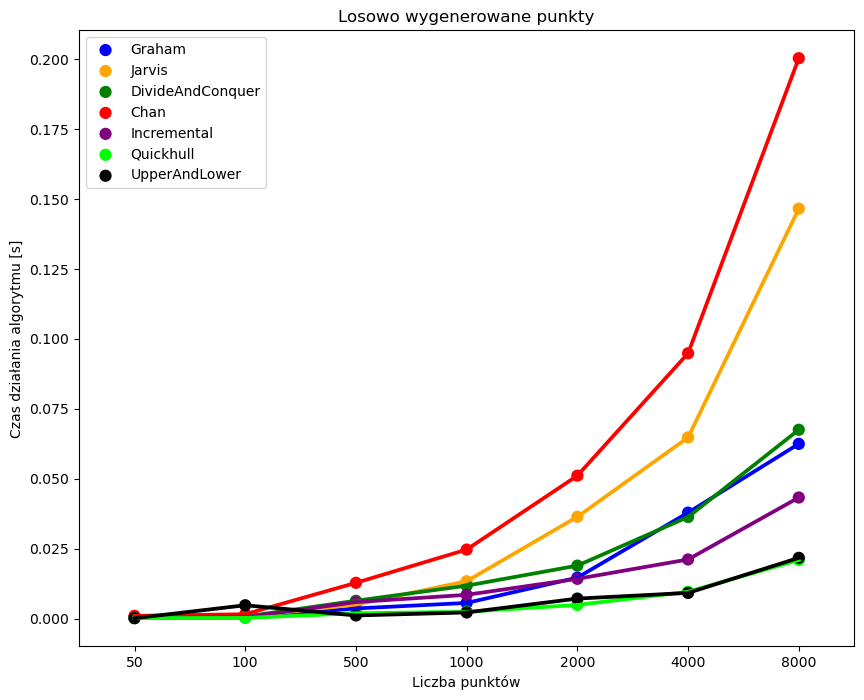
\includegraphics[scale=0.6]{./img/range.png}
\captionof{figure}{Wykres przedstawiający pomiar czasów działania algorytmów dla zbiorów typu range}

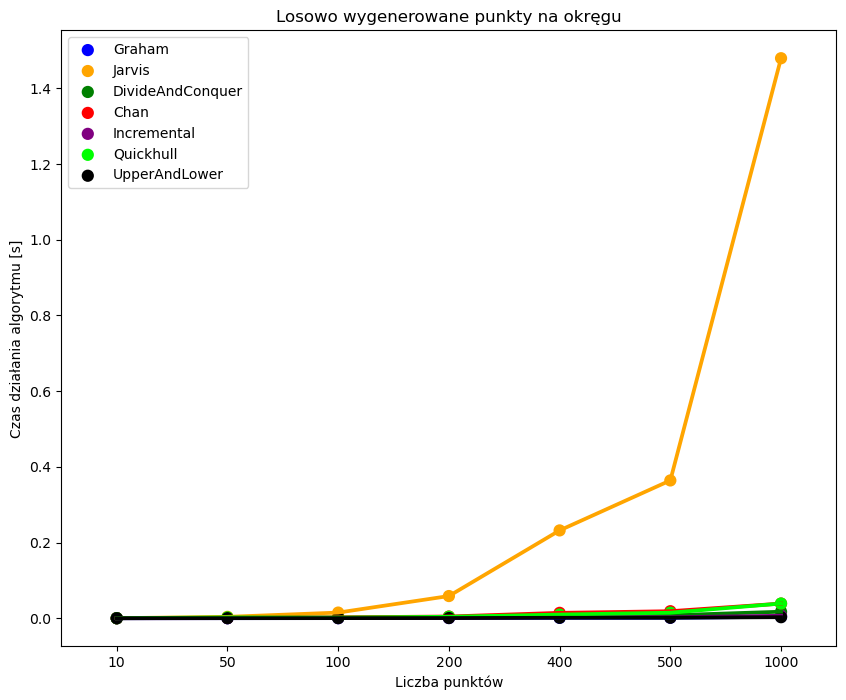
\includegraphics[scale=0.6]{./img/circle.png}
\captionof{figure}{Wykres przedstawiający pomiar czasów działania algorytmów dla zbiorów typu circle}

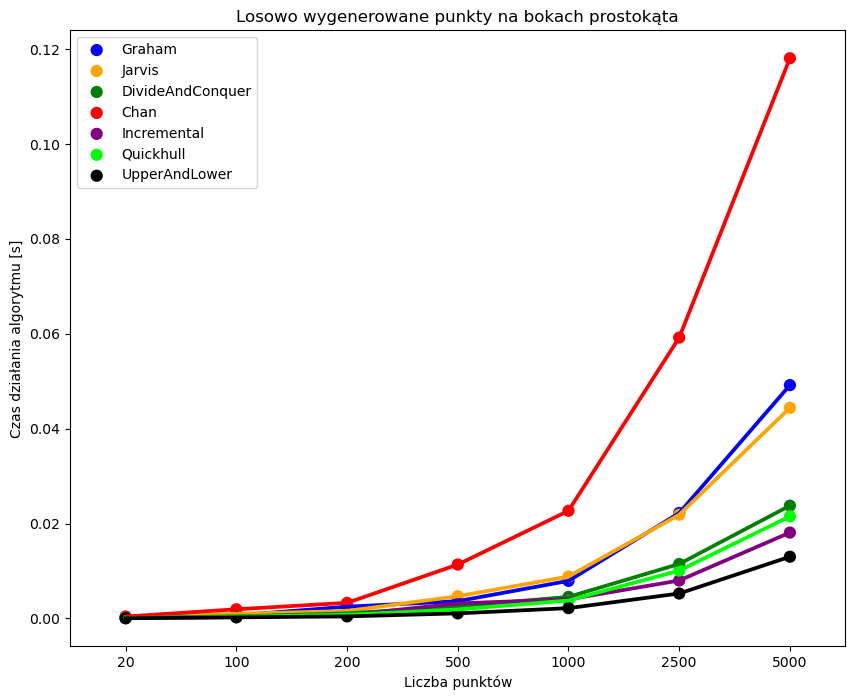
\includegraphics[scale=0.6]{./img/rectangle.png}
\captionof{figure}{Wykres przedstawiający pomiar czasów działania algorytmów dla zbiorów typu rectangle}

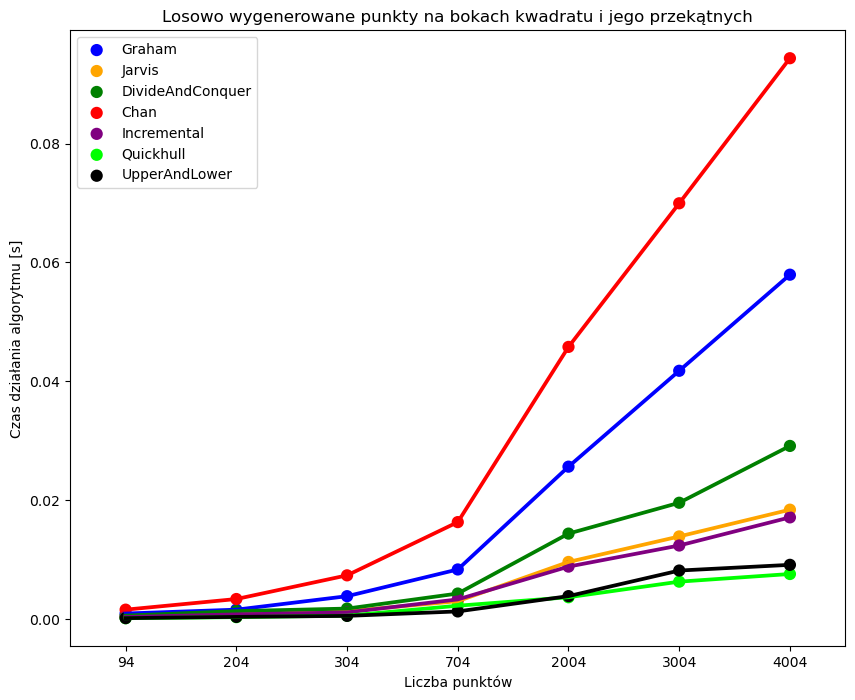
\includegraphics[scale=0.6]{./img/square.png}
\captionof{figure}{Wykres przedstawiający pomiar czasów działania algorytmów dla zbiorów typu square}
\end{center}
\end{document}